\section*{Exercise 1}
In this assignment, we implement the k-means algorithm for clustering the input data points. The whole source code of the project can be found in the Github repository \url{https://github.com/MazenAly/datamining}.

Clustering is considered as an unsupervised machine learning technique. That means there are no labels in the data that we need to predict, but it helps us get some insights about the input data.

We developed four methods for initializing the first $k$ cluster centroids (where $k$ is an input).
The first method is just choosing the first $k$ data points to be the centroids, the second one is randomized selections of the initial centroids, the third one is k-means++,
and the fourth method is using Gonzales’ algorithm to pick the initial centroids.

For each method, we run k-means for different values, $k \in {3,4,5}$, and in randomized methods, we experiment that 5 times. We visualize the results to get more understanding and learning experience as shown below. In figure \ref{clustering_result}, we shows the k-means clustering result on the dataset C2.txt with various initialization strategies and different values of $k$.

\begin{figure}[!htb]
\centering
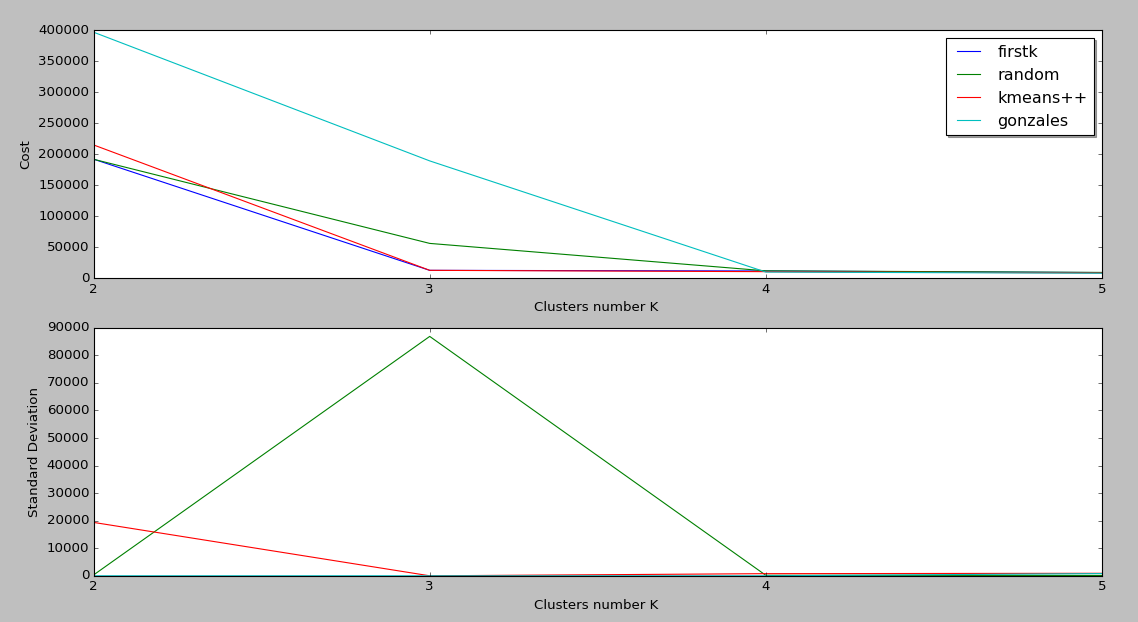
\includegraphics[width=0.9\textwidth]{shots/std_mean.png}
\caption{The average costs(top) and average Standard deviations(bottom) of several runs of k-means for different clusters numbers and using different methods of initialization.}
\label{std_mean}
\end{figure}

The top digram of figure \ref{std_mean} shows the average cost of 5 runs of each method of initialization for k-means for different number of clusters, we can see that Gonzales method has the worst average cost across all the methods for 2 and 3 clusters. Starting of 4, all the methods have similar costs on average. The reason for this is the distribution of the data points in the file C2, where there is an outlier point that is very far from all the other points. This point is thus always chosen by Gonzales' algorithm as a center of one of the clusters.

The bottom figure shows standard deviation of the costs across all the 5 runs. We can see that the random initialization can have higher standard deviation which means that one or more of the runs can be highly deviated from average of the runs.

\begin{figure}[!htb]
\centering
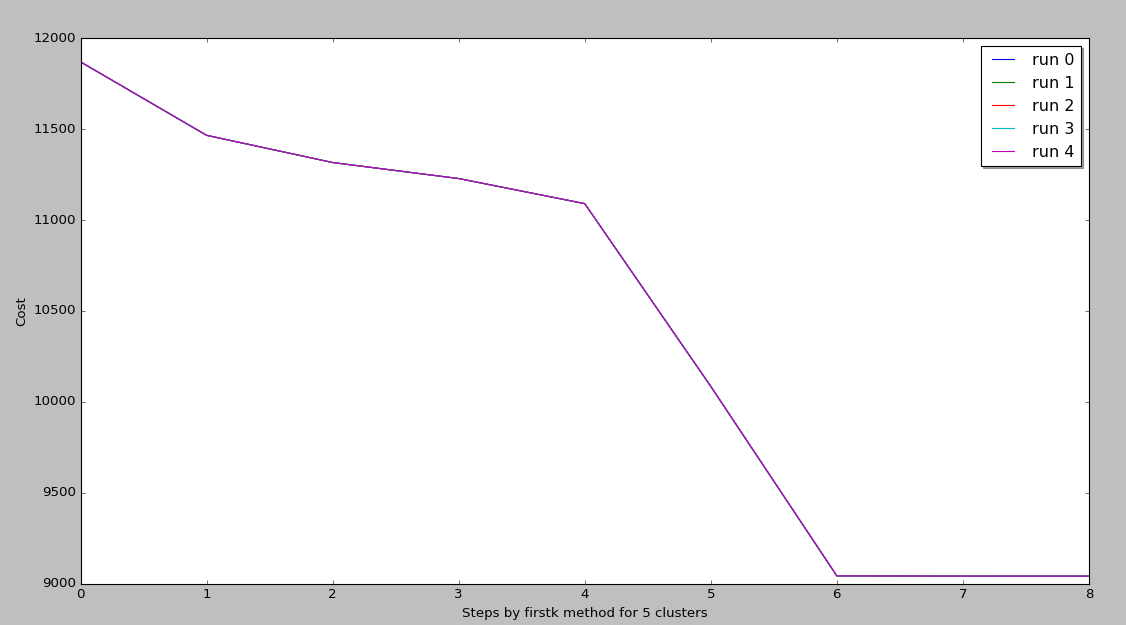
\includegraphics[width=0.9\textwidth]{shots/firstk5clusters.png}
\caption{Convergent rate of k-means using the first 5 points as initial centroids. }
\label{firstk5clusters}
\end{figure}

Figure \ref{firstk5clusters} shows the convergence rate of k-means algorithm using the first 5 points as the initial centroids. We can see that of course it will be the same for all the runs, because there are no randomizations.

Doing the same for the random method, we can see in figures \ref{random3clusters}, \ref{random4clusters} and \ref{random5clusters} that for 3,4 and 5 clusters we can see different rates of convergence in each of the 5 runs for each value of $k$, which shows that k-means algorithm is dependent on the initial centroids.

\begin{figure}[!htb]
\centering
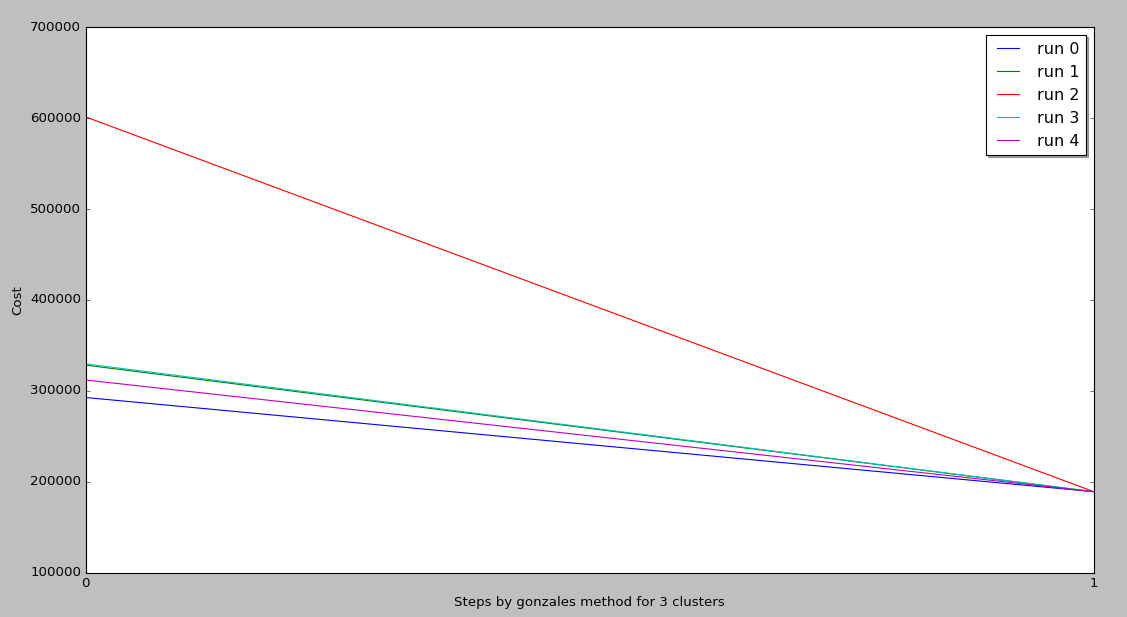
\includegraphics[width=0.9\textwidth]{shots/gonzales3clusters.png}
\caption{Convergence rate of k-means using initialization of Gonzales' algorithm and 3 clusters for 5 different runs }
\label{gonzales3clusters}
\end{figure}

\begin{figure}[!htb]
\centering
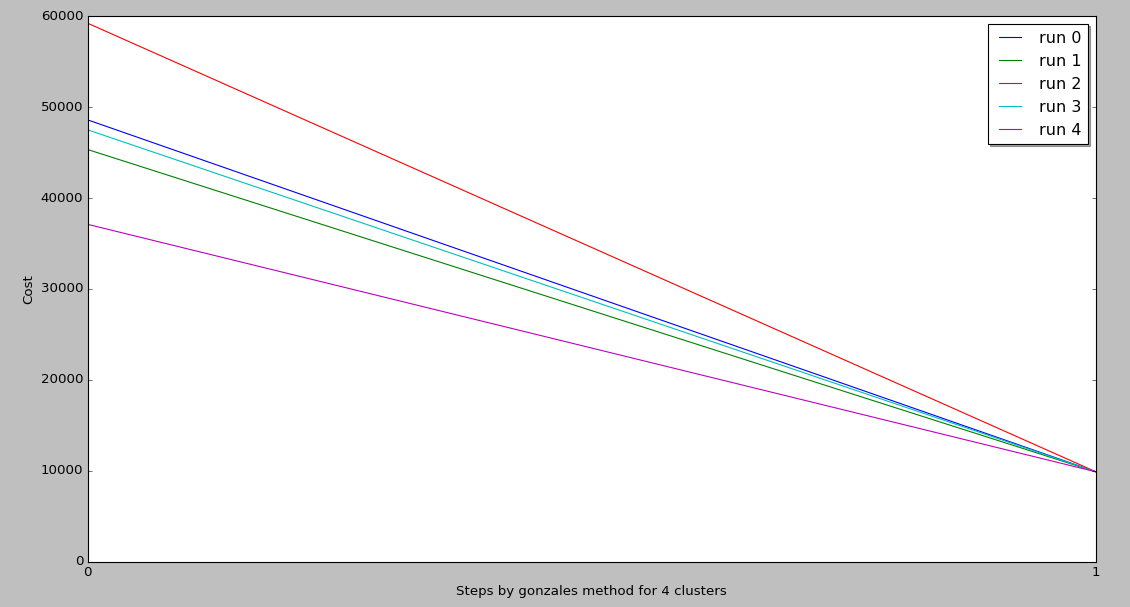
\includegraphics[width=0.9\textwidth]{shots/gonzales4clusters.png}
\caption{Convergence rate of k-means using initialization of Gonzales' algorithm and 4 clusters for 5 different runs  }
\label{gonzales4clusters}
\end{figure}

\begin{figure}[!htb]
\centering
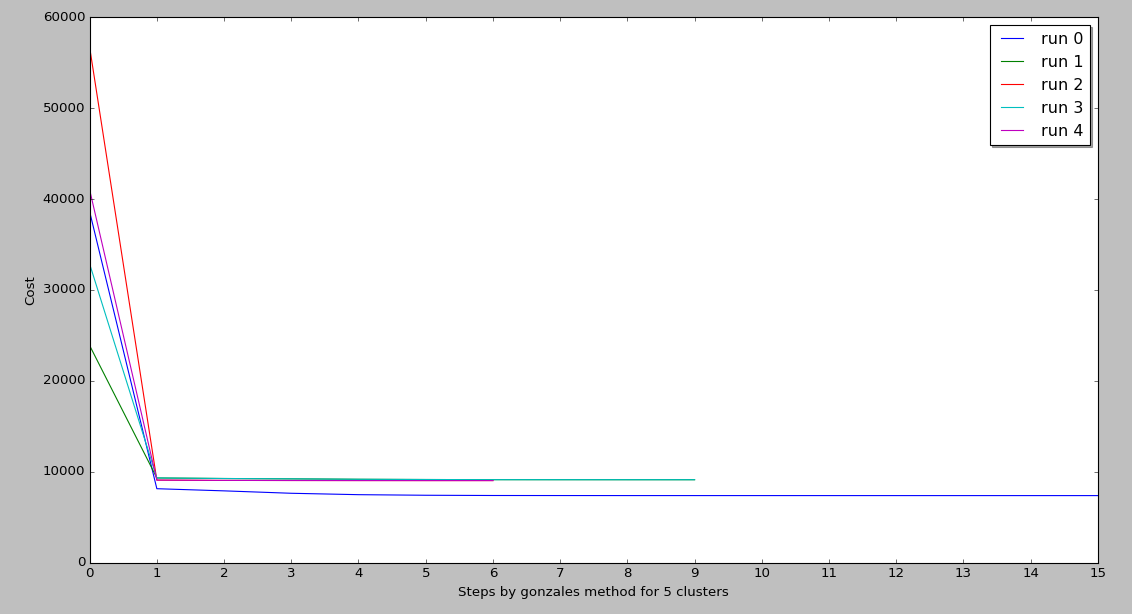
\includegraphics[width=0.9\textwidth]{shots/gonzales5clusters.png}
\caption{ Convergence rate of k-means using initialization of Gonzales' algorithm and 5 clusters for 5 different runs }
\label{gonzales5clusters}
\end{figure}

Figure \ref{gonzales3clusters} and \ref{gonzales4clusters} shows the convergence rate of k-means algorithm of 3 clusters using Gonzales's algorithm centers as the initial centroids, we can see it converged in just one step.

But for 5 clusters, Gonzales' algorithm convergence rates are diverse between 1 and 15 steps as in figure \ref{gonzales5clusters}.

\begin{figure}[!htb]
\centering
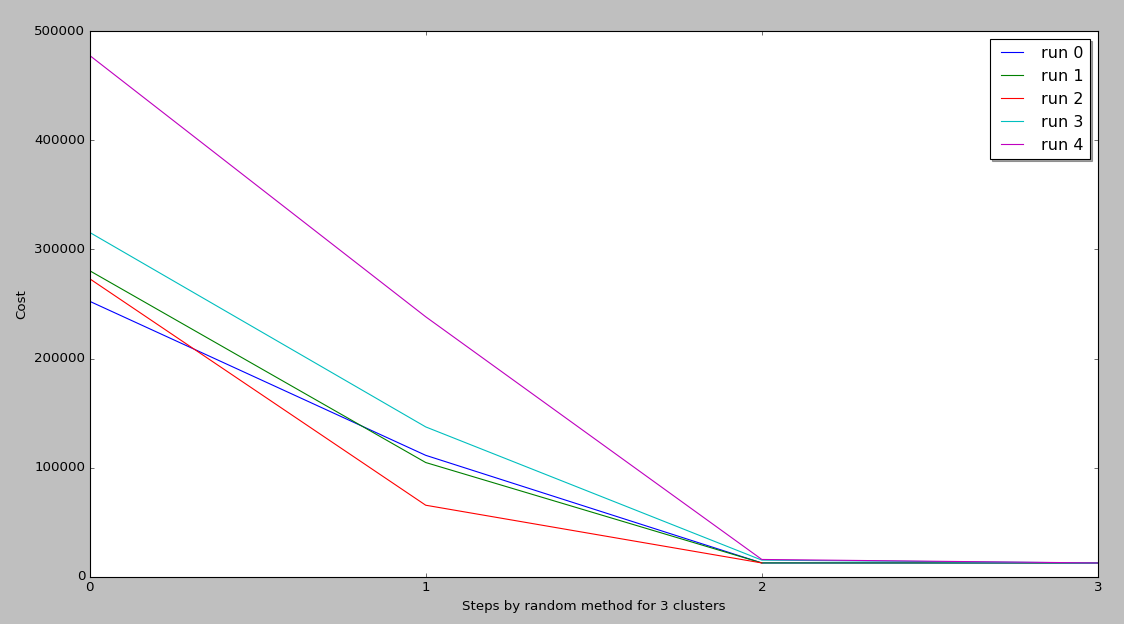
\includegraphics[width=0.9\textwidth]{shots/random3clusters.png}
\caption{ Convergence rate of k-means using random initialization and 3 clusters for 5 different runs }
\label{random3clusters}
\end{figure}

\begin{figure}[!htb]
\centering
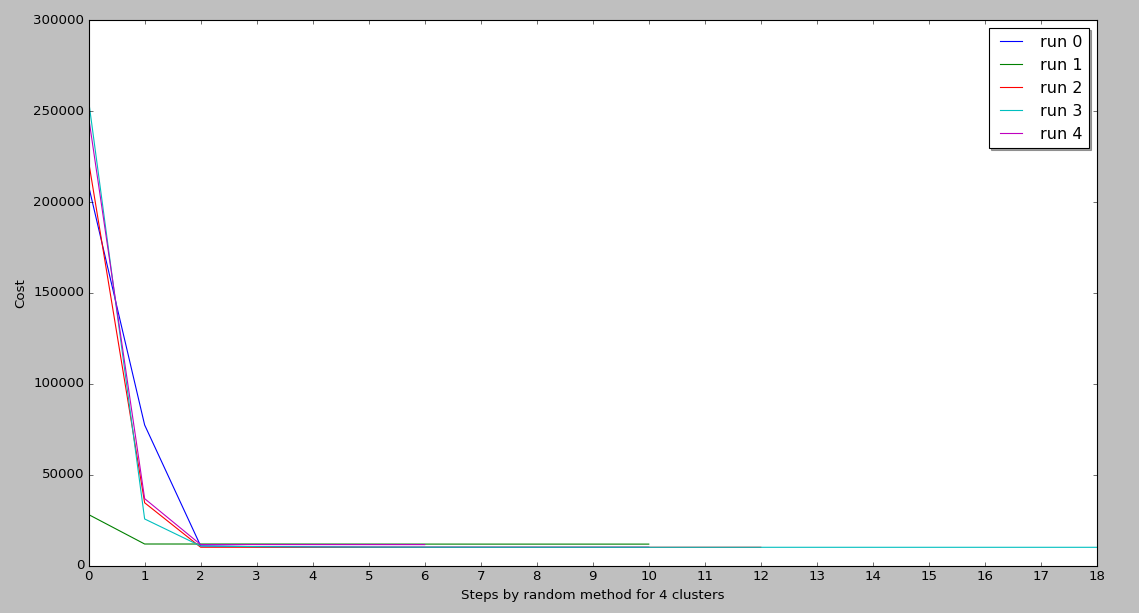
\includegraphics[width=0.9\textwidth]{shots/random4clusters.png}
\caption{ Convergence rate of k-means using random initialization and 4 clusters for 5 different runs }
\label{random4clusters}
\end{figure}

\begin{figure}[!htb]
\centering
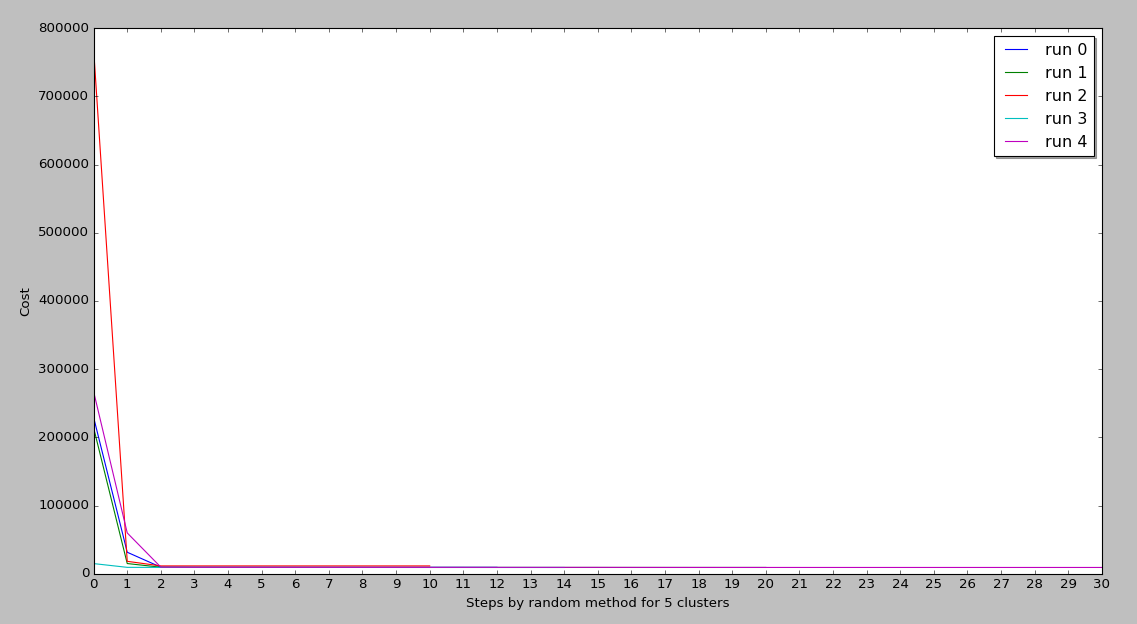
\includegraphics[width=0.9\textwidth]{shots/random5clusters.png}
\caption{ Convergence rate of k-means using random initialization and 5 clusters for 5 different runs  }
\label{random5clusters}
\end{figure}

For k-means++, we ran the algorithm 5 times for each different clusters number to visualize the convergence rate as in figures \ref{kmeans++3clusters} , \ref{kmeans++4clusters} and \ref{kmeans++5clusters}. We can see that the rates are also diverse across different runs but on average k-means++ converges faster due to the probabilistic 
strategy of choosing the first initial centroids.

\begin{figure}[!htb]
\centering
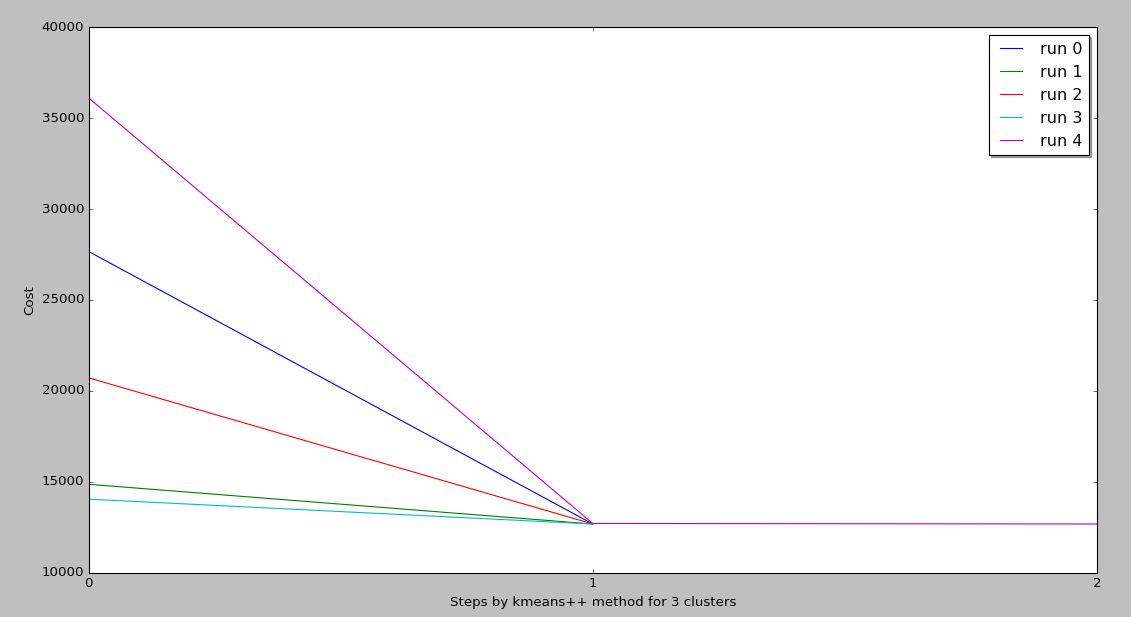
\includegraphics[width=0.9\textwidth]{shots/kmeans++3clusters.png}
\caption{ Convergence rate of k-means using kmeans++ initialization and 3 clusters for 5 different runs   }
\label{kmeans++3clusters}
\end{figure}

\begin{figure}[!htb]
\centering
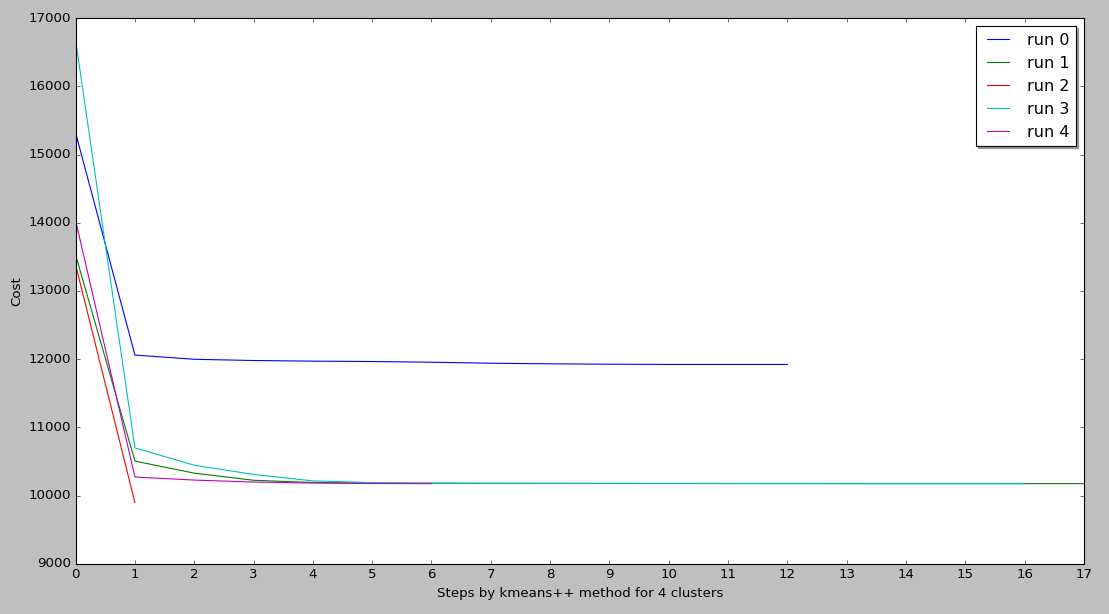
\includegraphics[width=0.9\textwidth]{shots/kmeans++4clusters.png}
\caption{Convergence rate of k-means using kmeans++ initialization and 4 clusters for 5 different runs  }
\label{kmeans++4clusters}
\end{figure}

\begin{figure}[!htb]
\centering
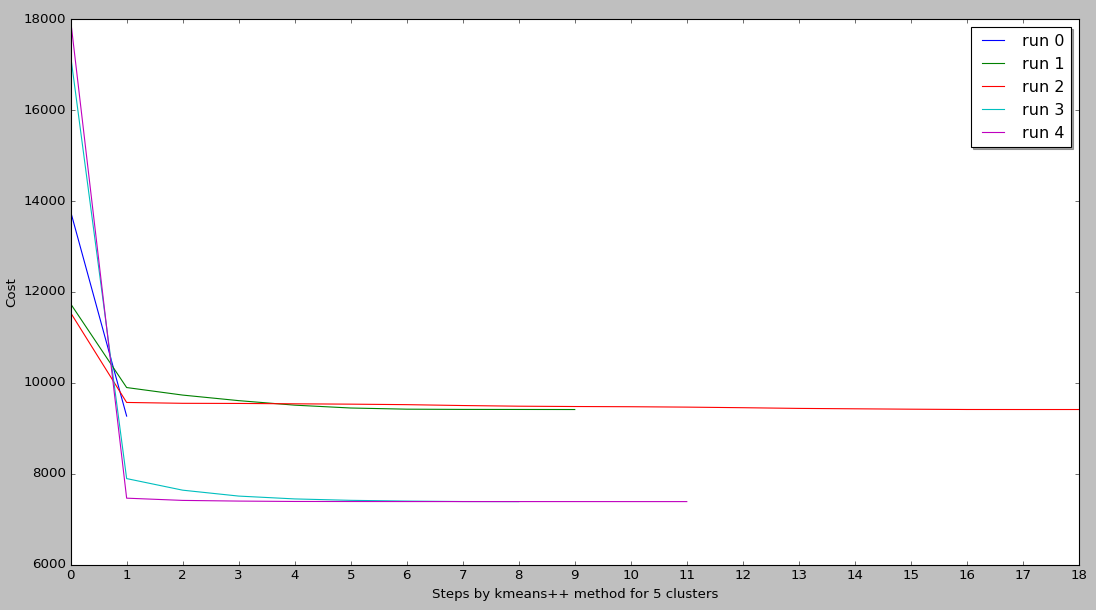
\includegraphics[width=0.9\textwidth]{shots/kmeans++5clusters.png}
\caption{ Convergence rate of k-means using kmeans++ initialization and 5 clusters for 5 different runs }
\label{kmeans++5clusters}
\end{figure}

Based on our experiments, k-means++ is the most robust implementation as it allows some weighted randomizations. The naive method of choosing the first $k$ centers depends on how good the data is originally sorted, which does not usually happen. The uniform randomization tries to overcome that weakness, but there are also (many) other bad configurations that can be selected randomly as well. For the Gonzales algorithm, we can take a look at figure \ref{clusters_gonz}. The noise is in its own cluster, and 2 meaningful clusters are grouped into only one. This example shows that using Gonzales algorithm for initializing k-means is not a good idea. This algorithm is very sensitive to noise as it always chooses the farthest point to be the next center.

\begin{figure}
  % hspace*{-0.2\textwidth}
  \begin{subfigure}{.33\textwidth}
    \centering
    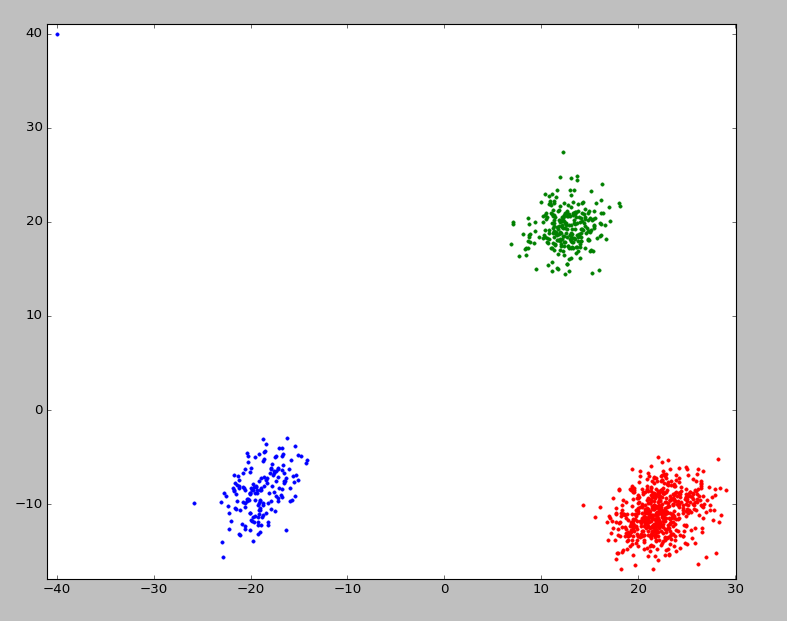
\includegraphics[width=\textwidth]{shots/clusters-firstk-3}
    \caption{Kmeans by picking first 3 points}
    \label{1-trilinear-compositing}
  \end{subfigure}
  \begin{subfigure}{.33\textwidth}
    \centering
    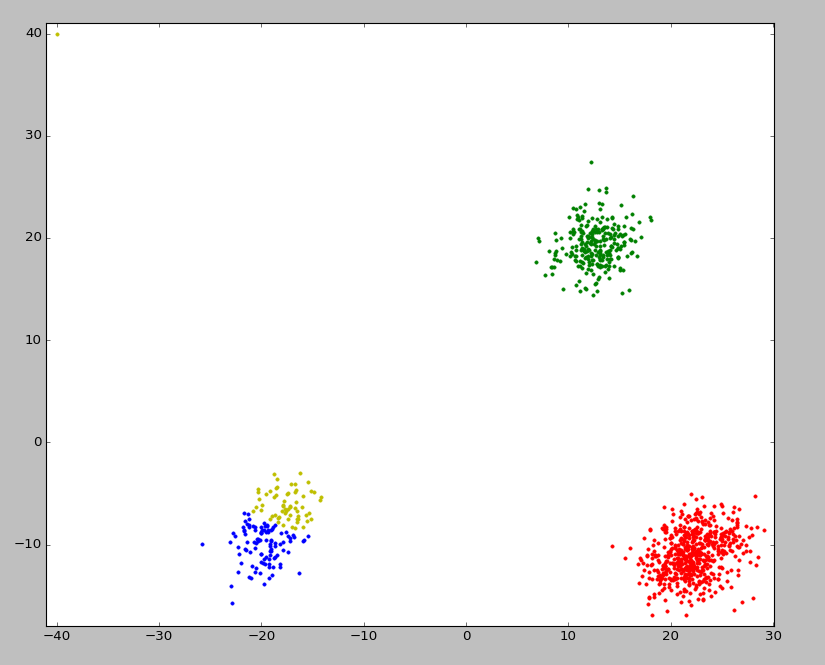
\includegraphics[width=\textwidth]{shots/clusters-firstk-4}
    \caption{Kmeans by picking first 4 points}
    \label{1-trilinear-compositing}
  \end{subfigure}
  \begin{subfigure}{.33\textwidth}
    \centering
    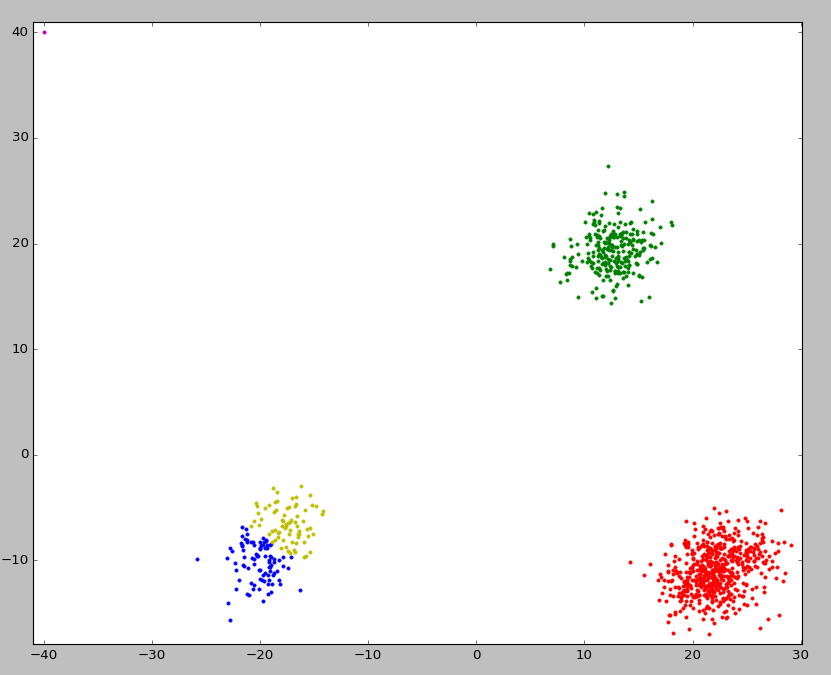
\includegraphics[width=\textwidth]{shots/clusters-firstk-5}
    \caption{Kmeans by picking first 5 points}
    \label{1-trilinear-compositing}
  \end{subfigure}
  \begin{subfigure}{.33\textwidth}
    \centering
    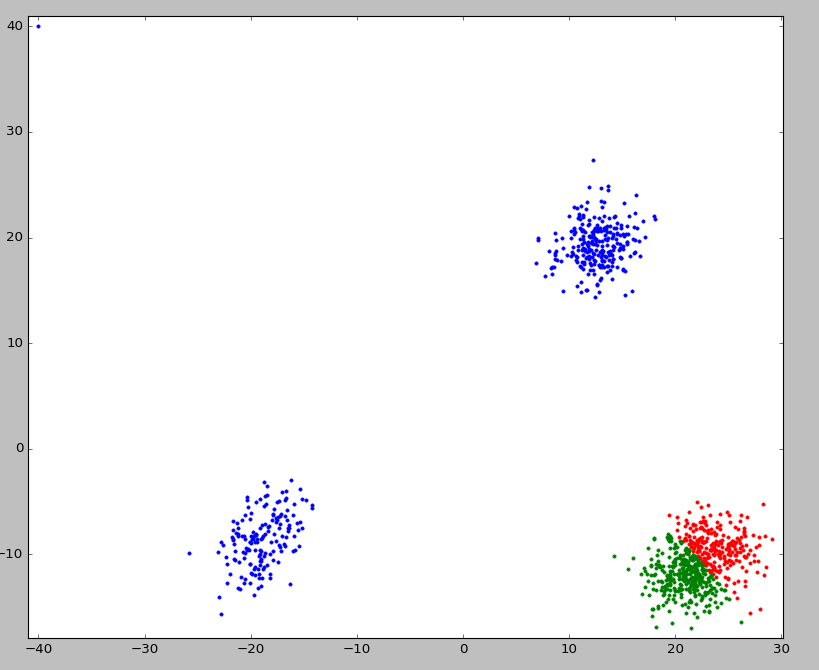
\includegraphics[width=\textwidth]{shots/clusters-random-3}
    \caption{Kmeans by picking first 3 random points}
    \label{1-trilinear-compositing}
  \end{subfigure}
  \begin{subfigure}{.33\textwidth}
    \centering
    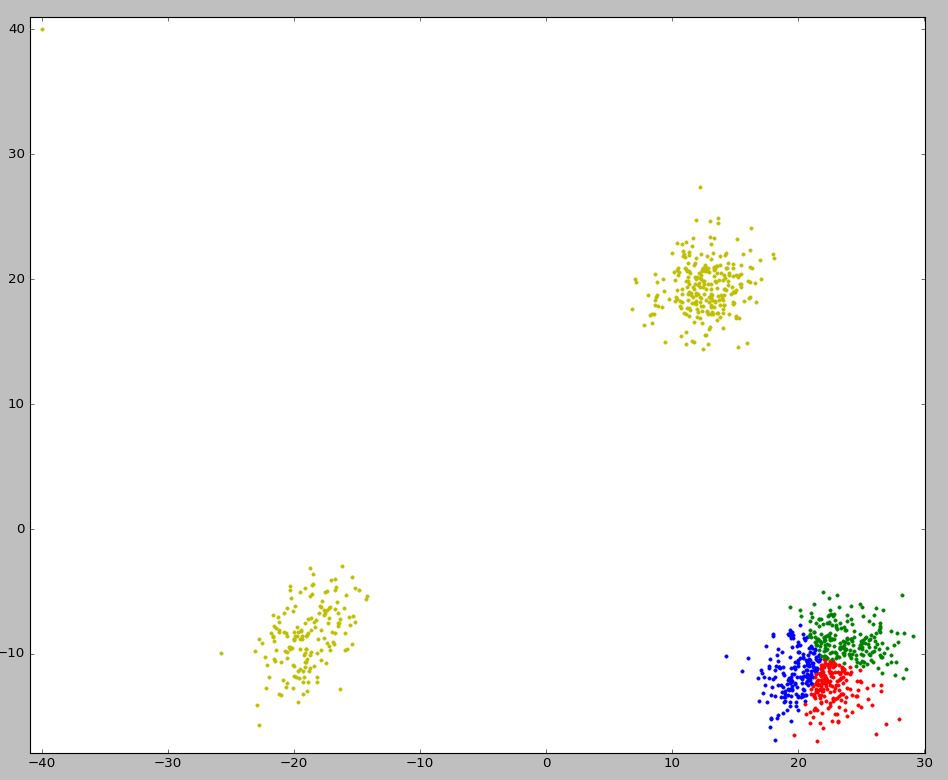
\includegraphics[width=\textwidth]{shots/clusters-random-4}
    \caption{Kmeans by picking first 4 random points}
    \label{1-trilinear-compositing}
  \end{subfigure}
  \begin{subfigure}{.33\textwidth}
    \centering
    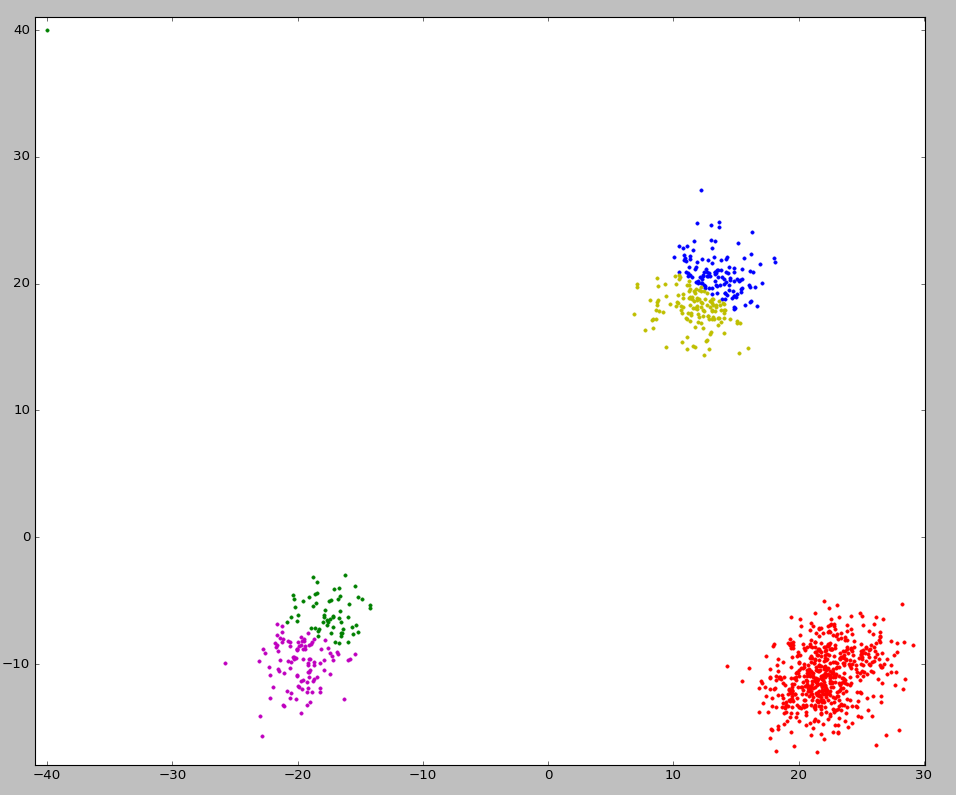
\includegraphics[width=\textwidth]{shots/clusters-random-5}
    \caption{Kmeans by picking first 5 random points}
    \label{1-trilinear-compositing}
  \end{subfigure}
  \begin{subfigure}{.33\textwidth}
    \centering
    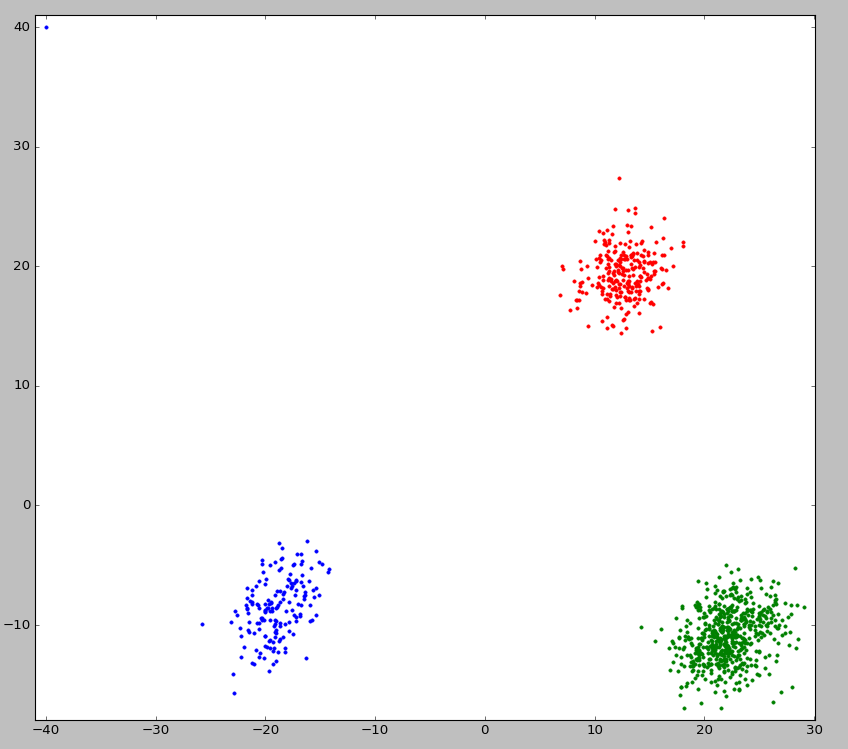
\includegraphics[width=\textwidth]{shots/clusters-kmeanspp-3}
    \caption{Kmeans++ with k = 3}
    \label{1-trilinear-compositing}
  \end{subfigure}
  \begin{subfigure}{.33\textwidth}
    \centering
    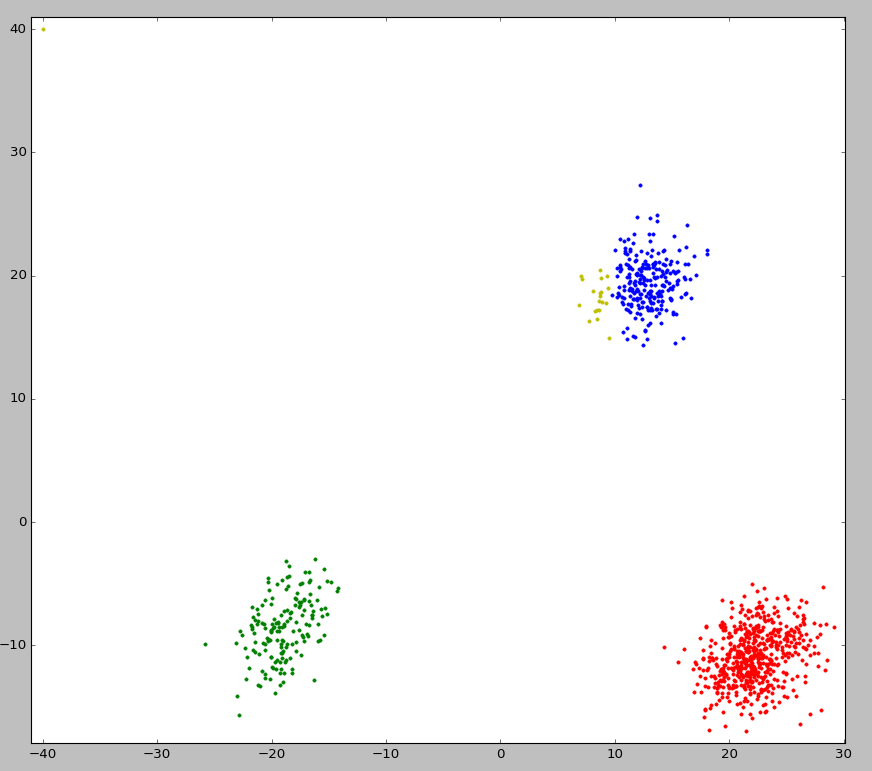
\includegraphics[width=\textwidth]{shots/clusters-kmeanspp-4}
    \caption{Kmeans++ with k = 4}
    \label{1-trilinear-compositing}
  \end{subfigure}
  \begin{subfigure}{.33\textwidth}
    \centering
    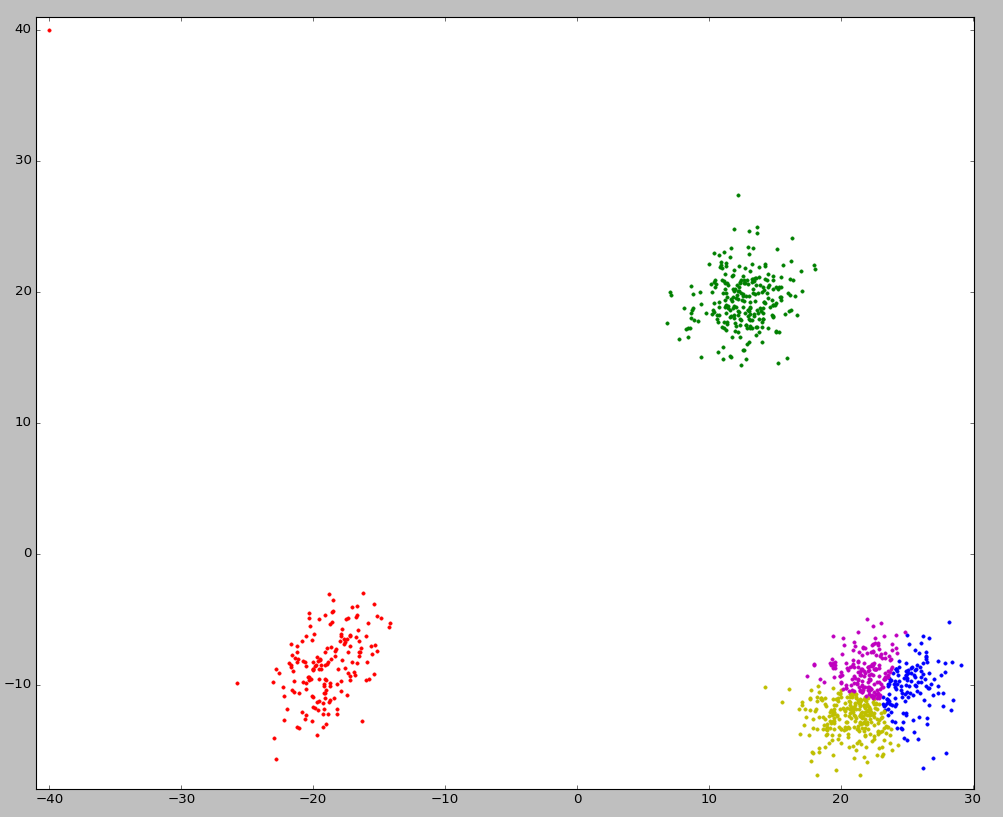
\includegraphics[width=\textwidth]{shots/clusters-kmeanspp-5}
    \caption{Kmeans++ with k = 5}
    \label{1-trilinear-compositing}
  \end{subfigure}
  \begin{subfigure}{.33\textwidth}
    \centering
    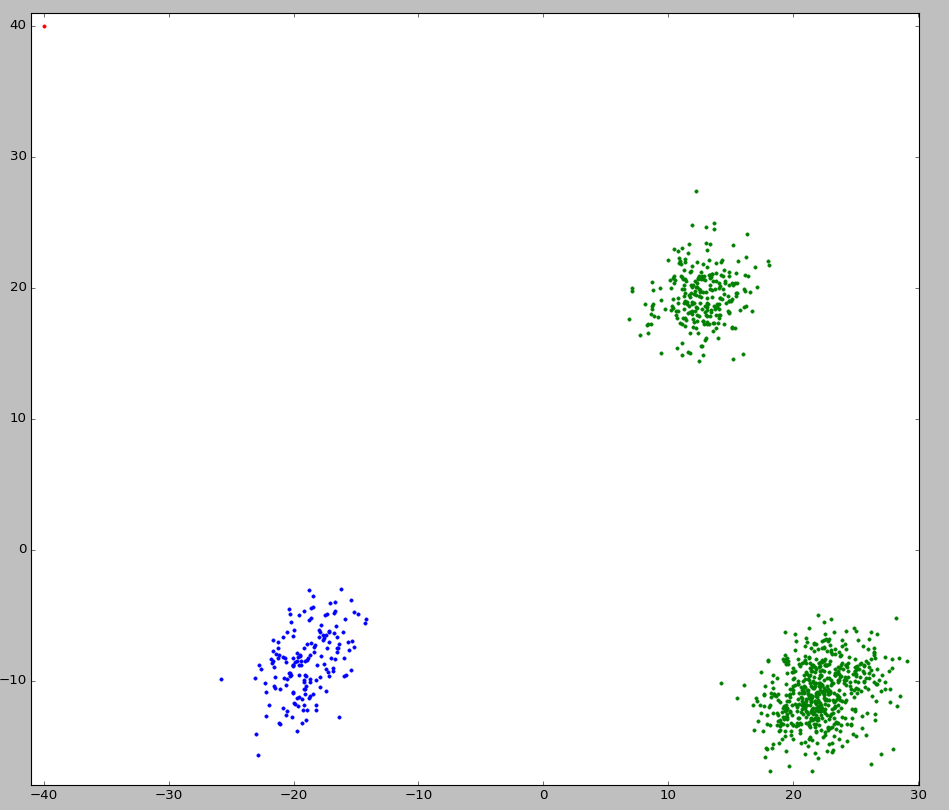
\includegraphics[width=\textwidth]{shots/clusters-gonz-3}
    \caption{Kmeans using Gonzales algorithm to choose the seeds, k = 3}
    \label{clusters_gonz}
  \end{subfigure}
  \begin{subfigure}{.33\textwidth}
    \centering
    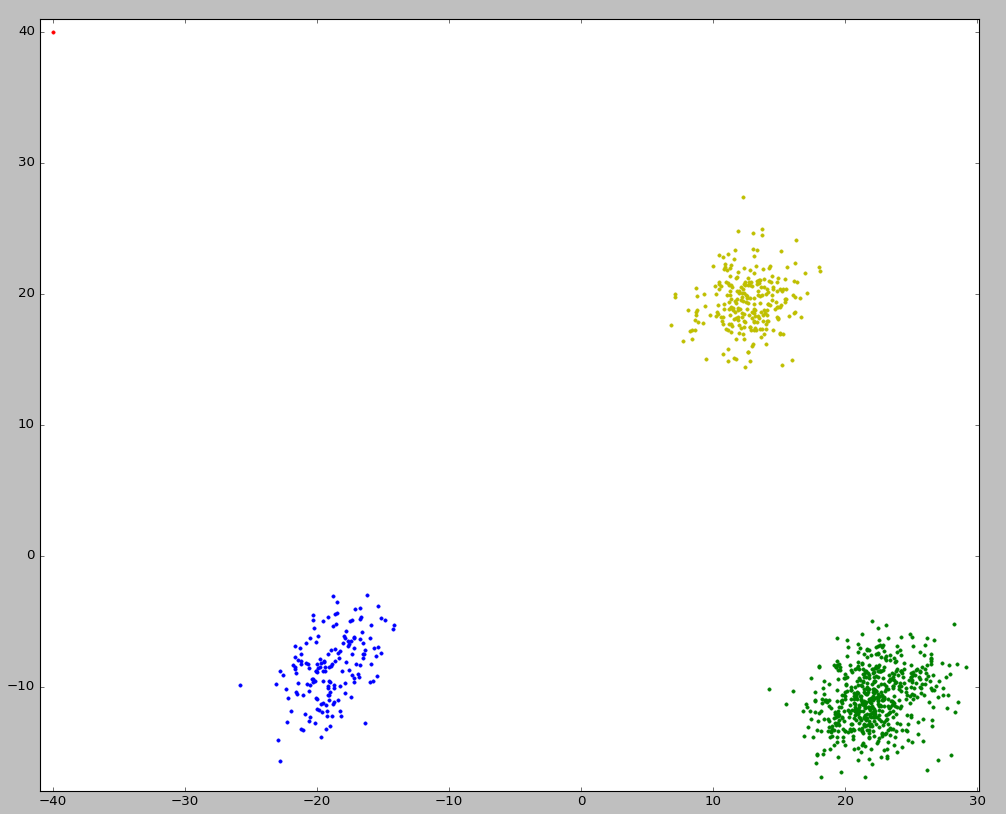
\includegraphics[width=\textwidth]{shots/clusters-gonz-4}
    \caption{Kmeans using Gonzales algorithm to choose the seeds, k = 4}
    \label{1-trilinear-compositing}
  \end{subfigure}
  \begin{subfigure}{.33\textwidth}
    \centering
    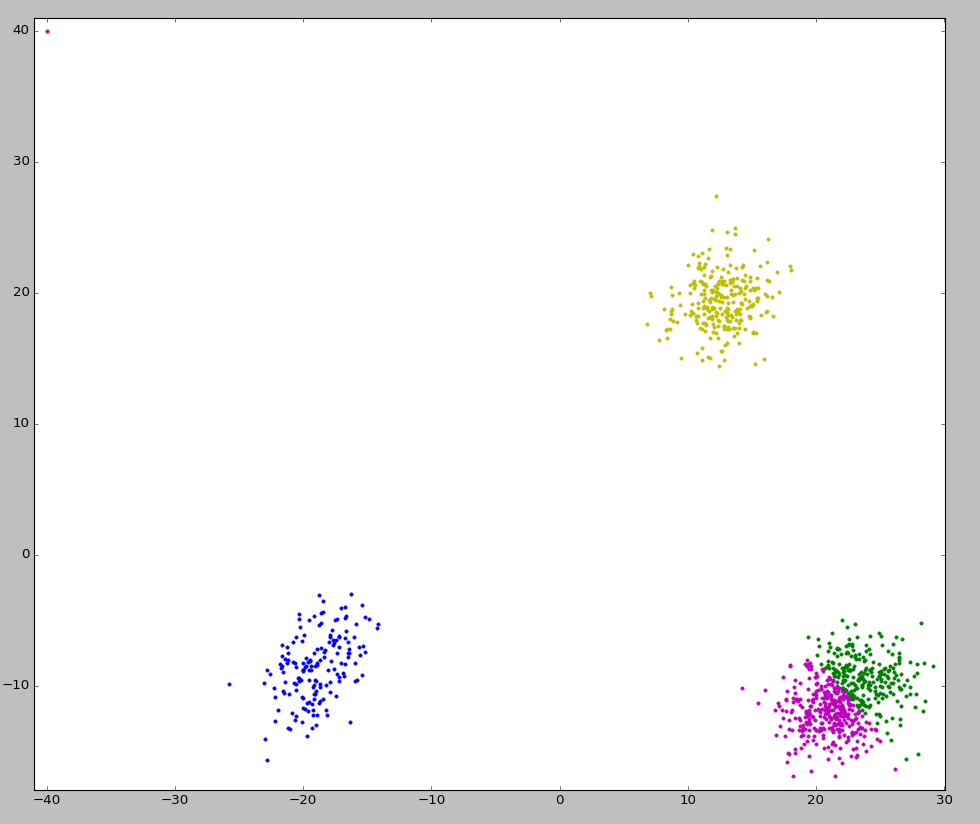
\includegraphics[width=\textwidth]{shots/clusters-gonz-5}
    \caption{Kmeans using Gonzales algorithm to choose the seeds, k = 5}
    \label{1-trilinear-compositing}
  \end{subfigure}
  \caption{K-means results with different settings}
  \label{clustering_result}
\end{figure}
